\documentclass[12pt]{article}
\usepackage{graphicx, amsmath}
\graphicspath{ {./} }
\setlength{\oddsidemargin}{0.25 in}
\setlength{\evensidemargin}{-0.25 in}
\setlength{\topmargin}{-0.6 in}
\setlength{\textwidth}{6.5 in}
\setlength{\textheight}{8.5 in}
\setlength{\headsep}{0.75 in}
\setlength{\parindent}{0 in}
\setlength{\parskip}{0.1 in}

\begin{document}
\thispagestyle{plain}
   \newpage
   \setcounter{page}{1}
   \noindent
   \begin{center}
   \framebox{
      \vbox{\vspace{2mm}
    \hbox to 6.28in { {\bf BioE 131: Intro to Computational Biology}
                        \hfill Fall 2020 }
       \vspace{4mm}
       \hbox to 6.28in { {\bf \Large \hfill Information Theory  \hfill} }
       \vspace{2mm}
       \hbox to 6.28in { {\it Professor: Ian Holmes \hfill} }
      \vspace{2mm}}
   }
   \end{center}
   {Notes written by Vikram Shivakumar}
   \vspace*{4mm}


\section{Introduction}
DNA sequences are fundamentally sequences of data that encode information for genes and regulatory signals. If we consider DNA sequences as data, one goal would be to quantify the amount of information in the sequence. To accomplish this, we can use concepts from \textbf{Information Theory}, a branch of mathematics, statistics, and computer science which explores how information is stored and quantified. in this note, we explore basic concepts from information theory and how they relate to data stored in nucleic acids, as well as various types of data compression.

\section{Shannon Entropy}
\subsection{Definitions}
\textbf{Shannon information}, introduced by Claude Shannon in 1948, describes the amount of information in a random variable. For a random variable $X$ and particular value $x$, the Shannon information would be the \textbf{negative log likelihood} of $x$:
$$h(x) = -\log_2P(x)$$
This value, $h(x)$, can be interpreted as the number of bits needed to represent the outcome $x$ from the random variable $X$. Consider for example a fair coin: the Shannon information of a heads outcome would be $-\log_2(.5) = 1$, meaning to encode the outcome of the coin flip, we would only need a single bit (0 or 1) to encode a heads, and likewise a tails.\\[10pt]
We can similarly calculate the \textbf{Shannon entropy} of a probability distribution by taking the sum of the Shannon information (number of bits) for each outcome, weighted by the \textit{likelihood} of the outcome:
$$S[P(x)] = \langle -\log_2P(x)\rangle_P = -\sum_{x\in X}P(x)\log_2P(x)$$
This weighted sum, $S[P(x)]$, is the Shannon entropy of the distribution, and represents the average number of bits needed to represent an outcome of $P(x)$. Looking again at the example of a fair coin, the Shannon entropy would again be $S[P(x)] = 1$, meaning in an \textit{ideal code}, only 1 bit is needed to encode the outcome of a fair coin flip (1 = heads, 0 = tails).\\[10pt]
Now lets take a look at a \textbf{biased} coin, where a heads occurs with probability $q$, and tails with $1-q$.
\begin{figure}[h]
    \centering
    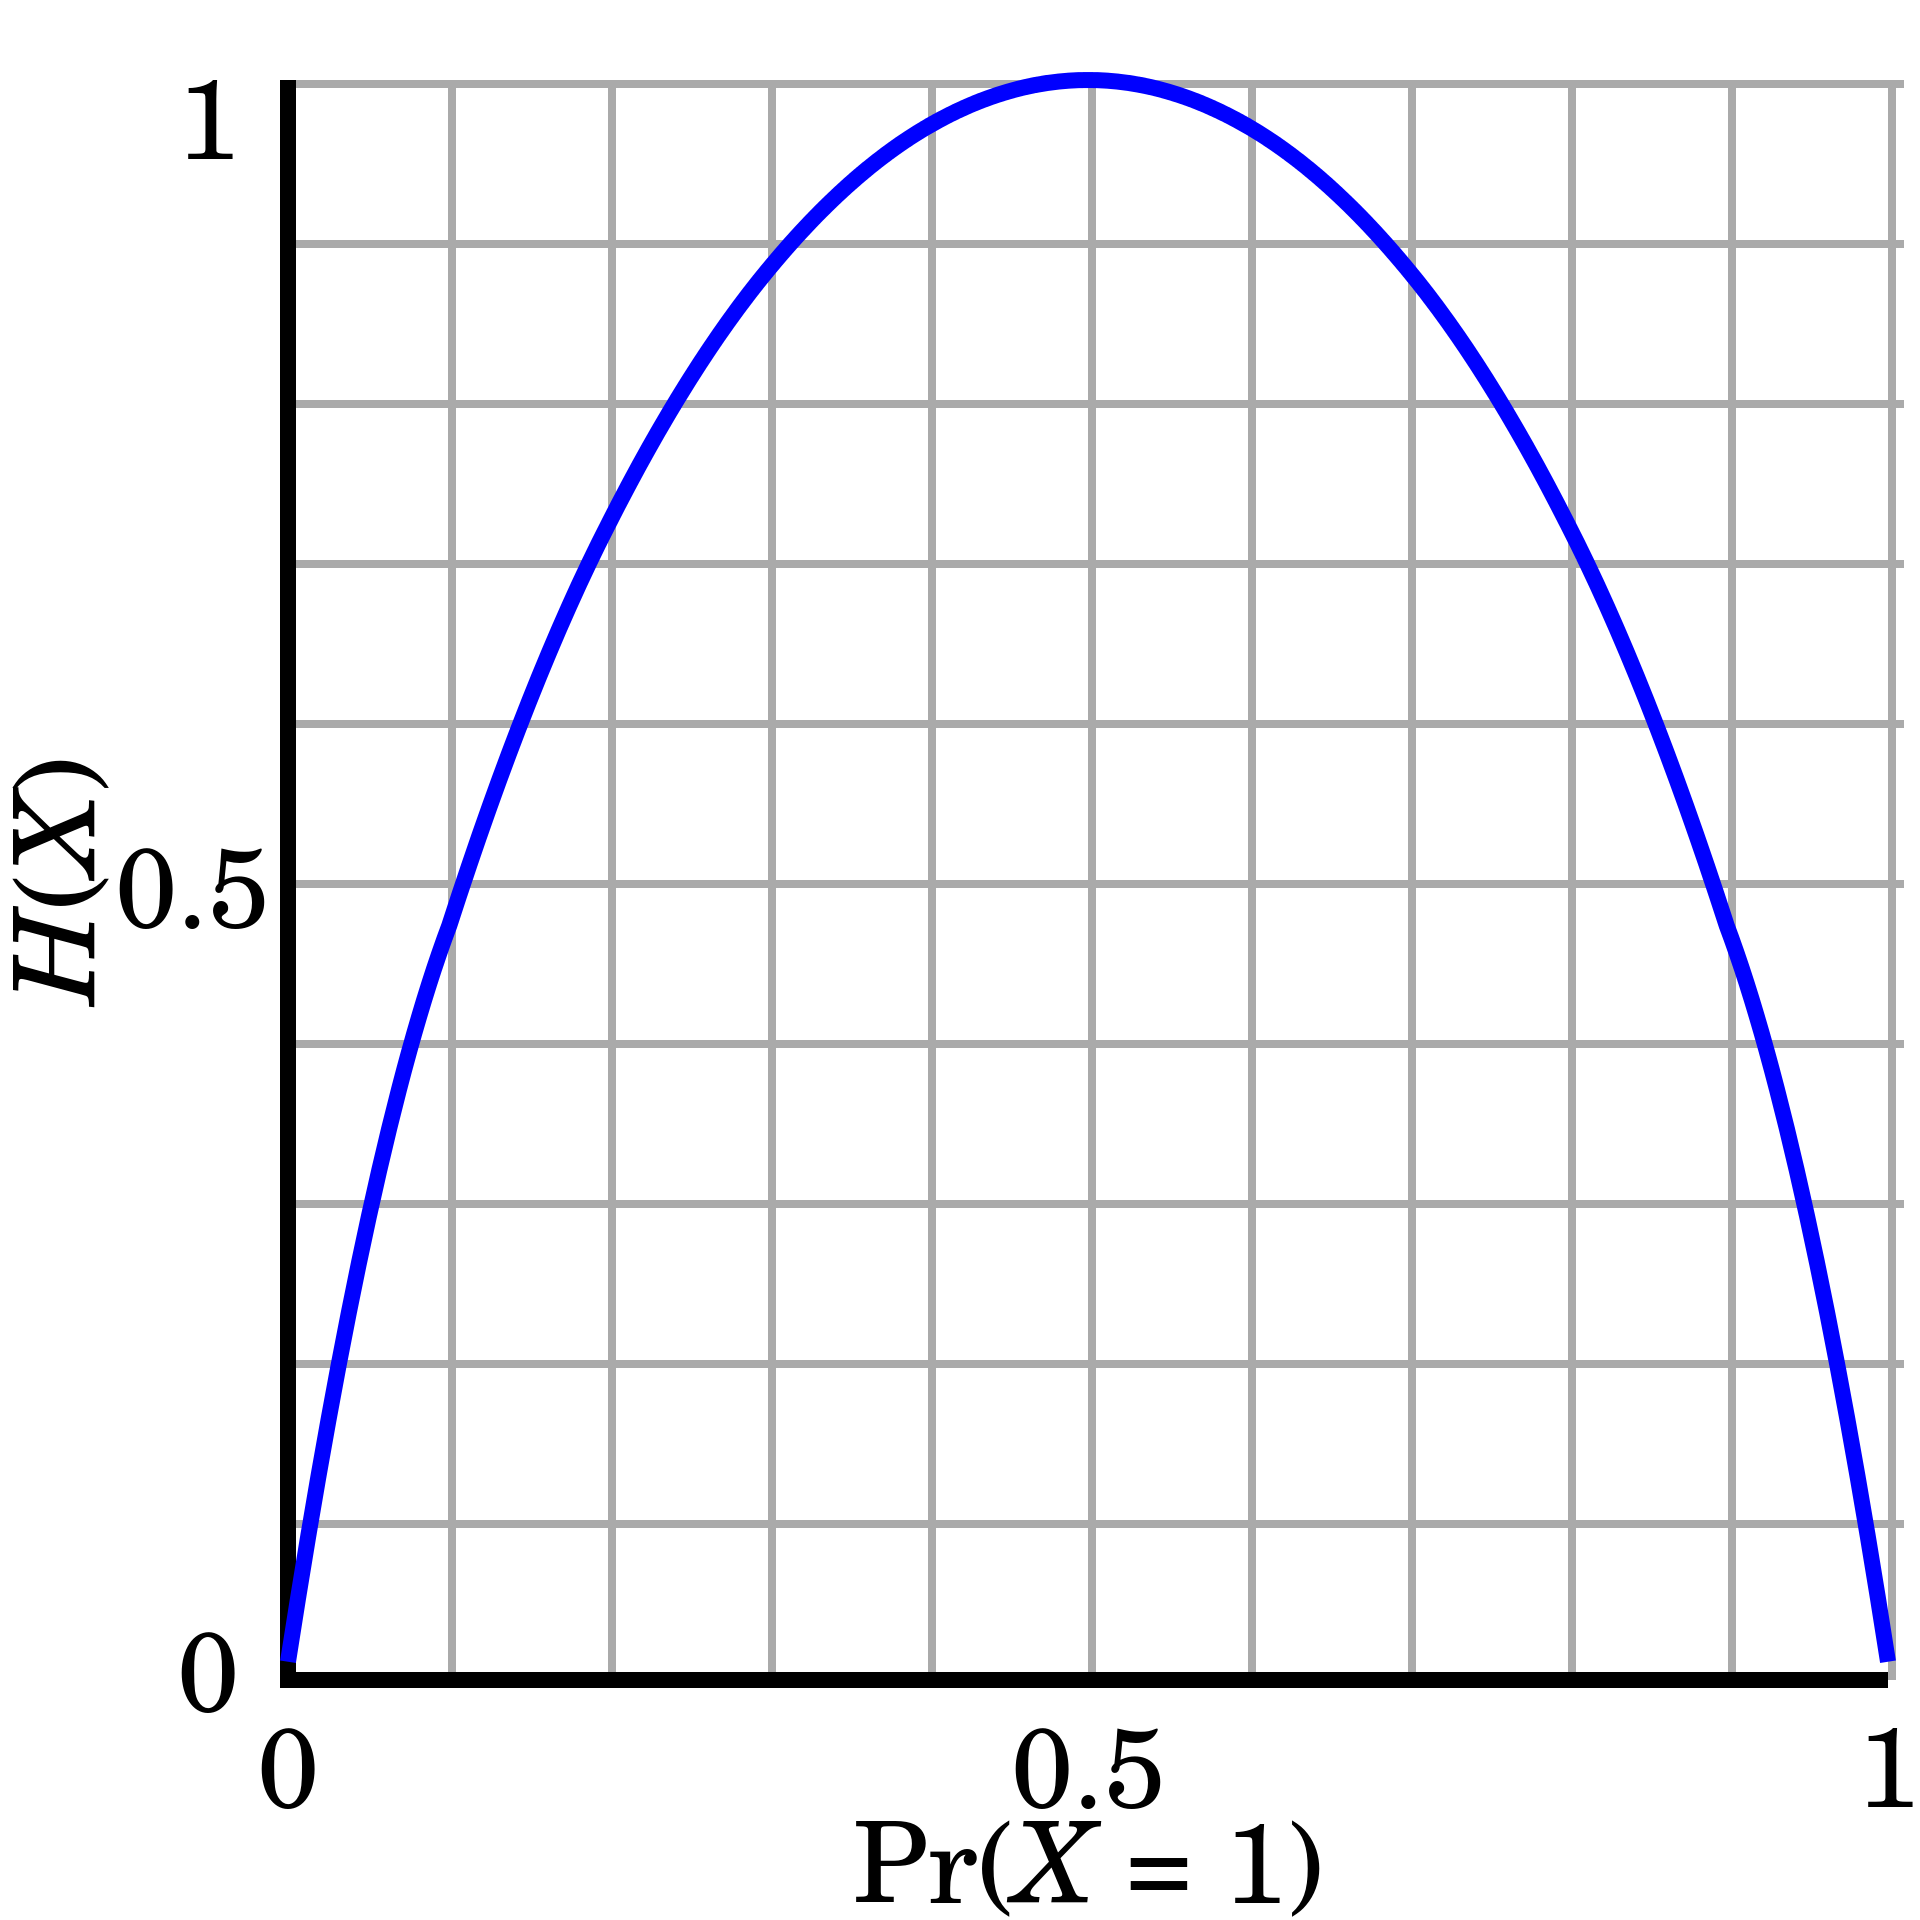
\includegraphics[width = .4\linewidth]{entropy.png}
    \caption{Entropy of a biased binary random variable}
    \label{fig:entropy}
\end{figure}
From figure \ref{fig:entropy}, the distribution has the most information when $q=0.5$, or the coin is fair. Extending beyond a binary example, the entropy of a random variable is maximized in a \textbf{uniform distribution}. Intuitively, when a random variable is heavily skewed to one outcome (i.e. the probability of heads is $q=0.99$), the RV is less uncertain, since the random variable almost always reliably outputs a single outcome, hence there is less entropy. The extreme case is when an outcome is certain ($P(x) = 1$), in which case there is no uncertainty, so no bits are needed to represent the outcome (it is always heads!), and the entropy is 0.\\[10pt]
In the case of a uniform distribution, the number of bits to encode each symbol is simply $\log_2(N)$, where N is the number of symbols in the distribution. This can be shown with the equation for Shannon information:
$$h(x) = -\log_2(P(x)) = -\log_2\left(\frac{1}{N}\right) = \log_2(N)$$
This is a special case of the idea that $h(x)$ represents the number of bits needed to encode a distribution in an \textit{ideal code} (Note: in reality, we can't encode each symbol with a fractional bit, so the number of bits needed would be $\log_2(N)$ rounded up).
\subsection{Entropy of DNA}
Using the formula for entropy, we can calculate the number of bits needed to encode a base in a DNA sequence: $\log_2(4) = 2$. Thus for a sequence where each base is has an equal 1/4 probability, we need 2 bits per nucleotide in an ideal code. However, what if A's occur with probability 1/2, C with probability 1/4, and G and T with probabilities 1/8? We can then compress the string to use less than 2 bits per base!
\begin{table}[h]
\centering
    
    \begin{tabular}{l|llll}
    Symbol    & A   & C   & G   & T   \\ \hline
    $P(x)$    & 1/4 & 1/4 & 1/4 & 1/4 \\
    $CP(x)$   & 00  & 01  & 10  & 11  \\
    $L(x;CP)$ & 2   & 2   & 2   & 2   \\ \hline
    $Q(x)$    & 1/2 & 1/4 & 1/8 & 1/8 \\
    $CQ(x)$   & 0   & 10  & 110 & 111 \\
    $L(x;CQ)$ & 1   & 2   & 3   & 3  
    \end{tabular}
    \caption{Encoding for uniform and non-uniform distributions}
    \label{tab:code}
\end{table}

In table \ref{tab:code}, we see the standard binary code for $P(x)$, and a modified code for the non-uniform $Q(x)$. We assign more bits to the infrequent nucleotides (G and T), and less bits to A, since it appears the more frequent.
\begin{figure}[h]
    \centering
    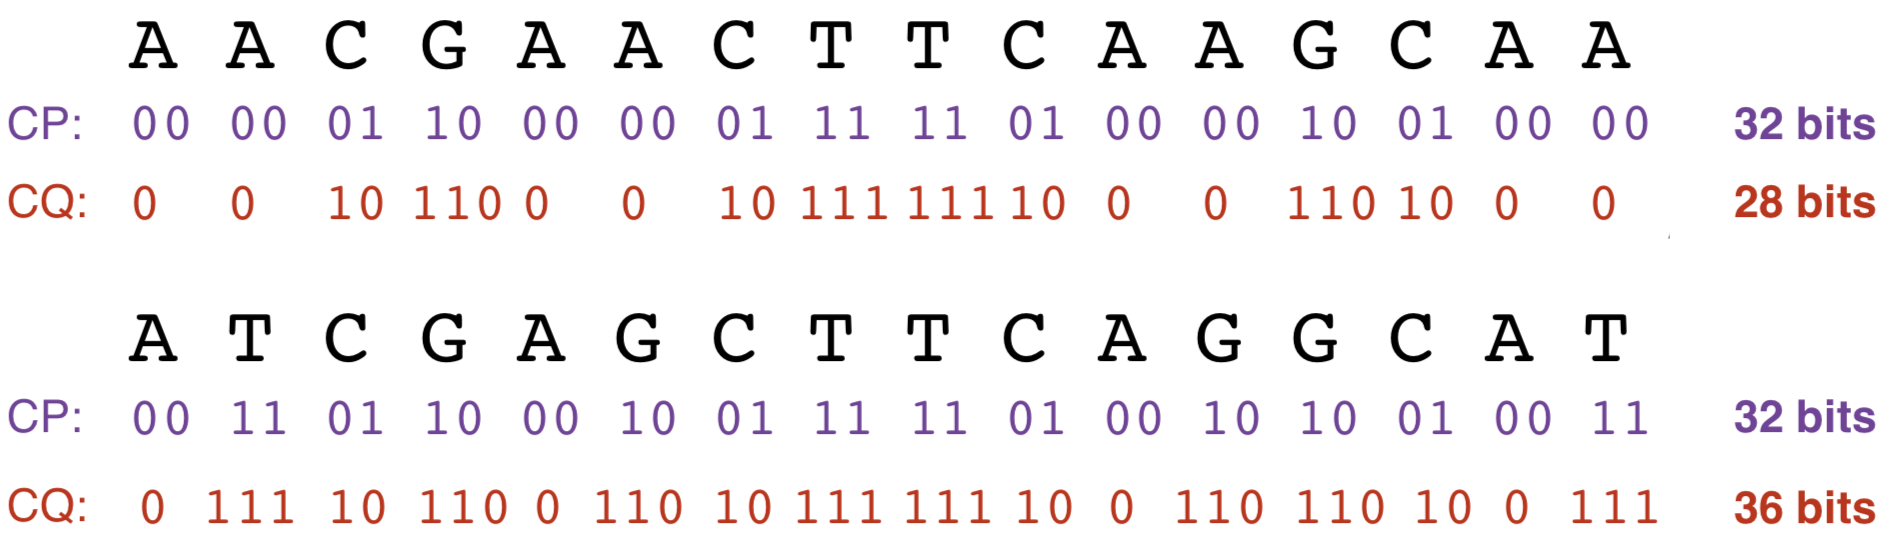
\includegraphics[width=.7\linewidth]{ideal_code.png}
    \caption{Encoding a non-uniform (top) and uniformly distributed (bottom) sequence}
    \label{fig:my_label}
\end{figure}
\\Here, $L(x; C)$ is the \textit{codeword length} for code $C$, and we define the expected codeword length as:
$$B(C;P) = \sum_xP(x)L(x;C)$$
We can calculate the expected codeword lengths for the codes and distributions in table \ref{tab:code}:
$$B(CP;P) = 2/4 + 2/4 + 2/4 + 2/4 = 2$$
$$B(CP;Q) = 2/2 + 2/4 + 2/8 + 2/8 = 2$$
$$B(CQ;P) = 1/4 + 2/4 + 3/4 + 3/4 = 9/4$$
$$B(CQ;Q) = 1/2 + 2/4 + 3/8 + 3/8 = 7/4$$
Recall that the Shannon entropy is the number of bits needed in an ideal code, thus if $B(C;P) = S[P]$, then $C$ is the ideal code for $P(x)$. We see here that using the code $CQ$ on distribution $P(x)$ is \textit{wasteful}, since it uses more bits on average than the \textit{ideal} code!\\[10pt]
In general, assuming $C$ represents the ideal code for $P(x)$, $B(CQ; P) \geq B(CP;P)$, and likewise, $B(CP;Q) \geq B(CQ;Q)$. Essentially, \textit{no code can do better than the ideal code}! (see the Kraft-McMillan inequality)
\subsection{Unique Decodability}
The codes in the previous section are \textbf{uniquely decodable}, in that given an encoded sequence, decoding only yields one message. These codes are also examples of \textbf{prefix codes}, which are always uniquely decodable. A prefix code is one in which no code is a prefix of another.\\[10pt]
For example, if symbol A is encoded with ``0", symbol B with ``1", and symbol C with ``01", the encoded message ``01" could be decoded as ``AB" or just ``C"! This ambiguity is a result of a non-prefix code, where the code for symbol A is a prefix of the code for symbol C.
\subsection{Relative entropy}
The \textbf{relative entropy} (also known as the \textbf{Kullback-Leibler distance}) of two distributions $P(x)$ and $Q(x)$ is defined as:
$$D(P||Q) = \sum_{x\in X}P(x)\log\frac{P(x)}{Q(x)} = \langle\log\frac{P(x)}{Q(x)}\rangle_p$$
(Note: $D(P||Q) \neq D(Q||P)$ in general). The relative entropy represents the \textit{distance} between two distributions, or the inefficiency of using the code for $P(x)$ on a sequence from $Q(x)$. Thus the relative entropy describes the relative saving (or wastage) of using a different code, and thus can be calculated using codeword lengths:
$$D(P||Q) = B(CQ;P) - B(CP;P)$$
Gibbs' inequality states that the relative entropy $D(P||Q) \geq 0$, which goes back to the idea that no code can outperform the \textit{ideal} code. In the equation above, no code $CQ$ can beat the ideal $CP$, so the difference in codeword lengths will always be positive.
\subsection{Mutual Information}
The mutual information of two random variables $x$ and $y$ represents the amount of information that each variable conveys about the other, and can be calculated using the following equation:
$$I(x;y) = \sum_x\sum_yp(x,y)\log\left(\frac{p(x,y)}{p(x)p(y)}\right) = D(p(x,y)||p(x)p(y))$$
Mutual information measures how efficient compressing both distributions as a single combined symbol would be versus compressing them separately. Unlike relative entropy, the mutual information is symmetric. It can be calculated using Shannon entropies as well:
$$I(x;y) = S(x) + S(y) - S(x,y)$$
Consider for example a multiple alignment of RNA sequences. 
\begin{figure}[h]
    \centering
    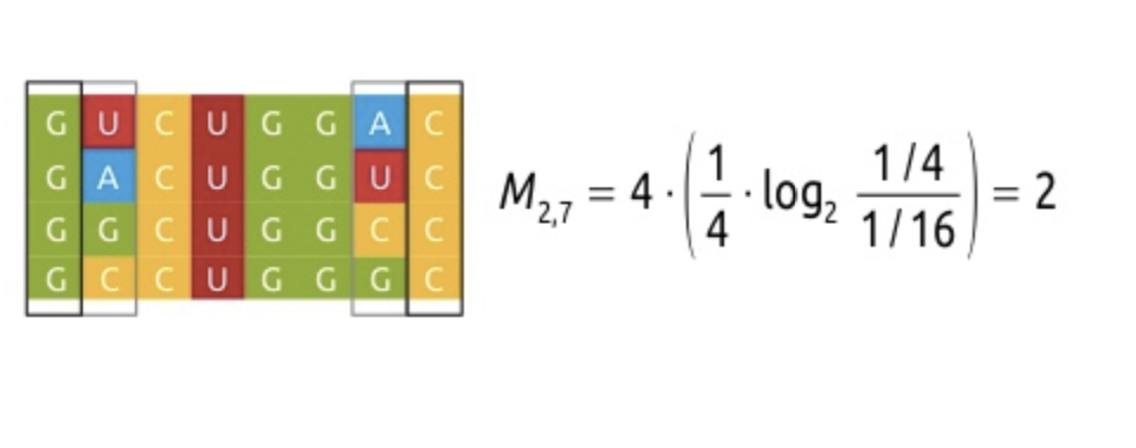
\includegraphics[width = .7\linewidth]{mutual.png}
    \caption{Example RNA alignment and mutual information calculation}
    \label{fig:mutual}
\end{figure}
Each column of the alignment represents the nucleotide distribution at a single position of the RNA sequence. Due to RNA structure, a mutation at one position often leads to a mutation at another base-paired position to maintain a fold-back structure. As a result, these two columns would have a high mutual information, since they are highly correlated.
\subsection{Conditional entropy}
The last type of entropy is conditional entropy, which measures the information content of a random variable $x$ given another random variable $y$, similar to a conditional probability:
$$S(x|y) = S(x,y) - S(y)$$
Thus we can relate mutual information to Shannon entropy and conditional entropy using the following equation:
$$I(x;y) = S(x) + S(y) - S(x,y)$$
$$I(x;y) = S(x) - S(x|y) = S(y) - S(y|x)$$

\section{Compression Schemes}
Now let's take a look at a few compression schemes that attempt to encode information as efficiently as possible (though never better than the \textit{ideal code}!)
\subsection{Binary/Unary Encoding}
We have already seen an example of a binary encoding, which takes $\log_2(N)$ bits, where there are $N$ symbols to encode. Binary encoding is ideal if all the symbols are uniformly distributed and N is a power of 2, for example in DNA, if each base is uniformly distributed.\\[10pt]
Unary encoding encodes each symbol as a run of 0s, followed by a delimiter 1. For example, to encode the number ``123", we would output ``010010001". This code is ideal if $P(x) = 2^{-x}$, or the probability distribution is geometric.
\subsection{Elias Gamma coding}
Elias gamma coding combines unary and binary encoding to encode integers. First, $N = \left \lfloor{\log_2x}\right \rfloor $ is calculated, the largest power of 2 less than $x$. the encoding is then $N$ consecutive 0s, followed by the binary representation of $x$. Thus $N$ is represented by unary encoding, and the remaining $N$ \textit{bits} of $x$ are represented with binary. This coding scheme is efficient if small values are more frequent than large values, and if the largest value to be encoded is not known ahead of time.
\subsection{Truncated binary encoding}
Truncated binary encoding can be used for sets of symbols that are not exactly a power of 2 in size. Similar to Elias gamma, $k = \left \lfloor{\log_2x}\right \rfloor $ is first calculated. Then we set $U = 2^{k + 1} - n$. We assign the first $U$ items in the set with a $k$ length binary encoding. Then we assign the remaining items the \textit{last} $n-U$ binary encodings of size $k+1$. This ensures a \textbf{prefix code}, since the last $n-U$ binary encodings of size $k+1$ are simply the unused $k$-length ancodings, with an extra bit added at the end!

\subsection{Golomb coding}
Golomb coding is a scheme that is ideal for geometrically distributed sets of symbols. First, for symbol $N$, $q = \left \lfloor{N / M}\right \rfloor $ and $r = N \mod M$ are calculated. The quotient $q$ is encoded with unary encoding. The remainder $r$ is then encoded using truncated binary encoding.
\subsection{Huffman coding}
Huffman coding uses a binary tree to build the code for each symbol, where the symbols are at the leaves of the tree, and the codes are represented by paths.
\begin{figure}[h]
    \centering
    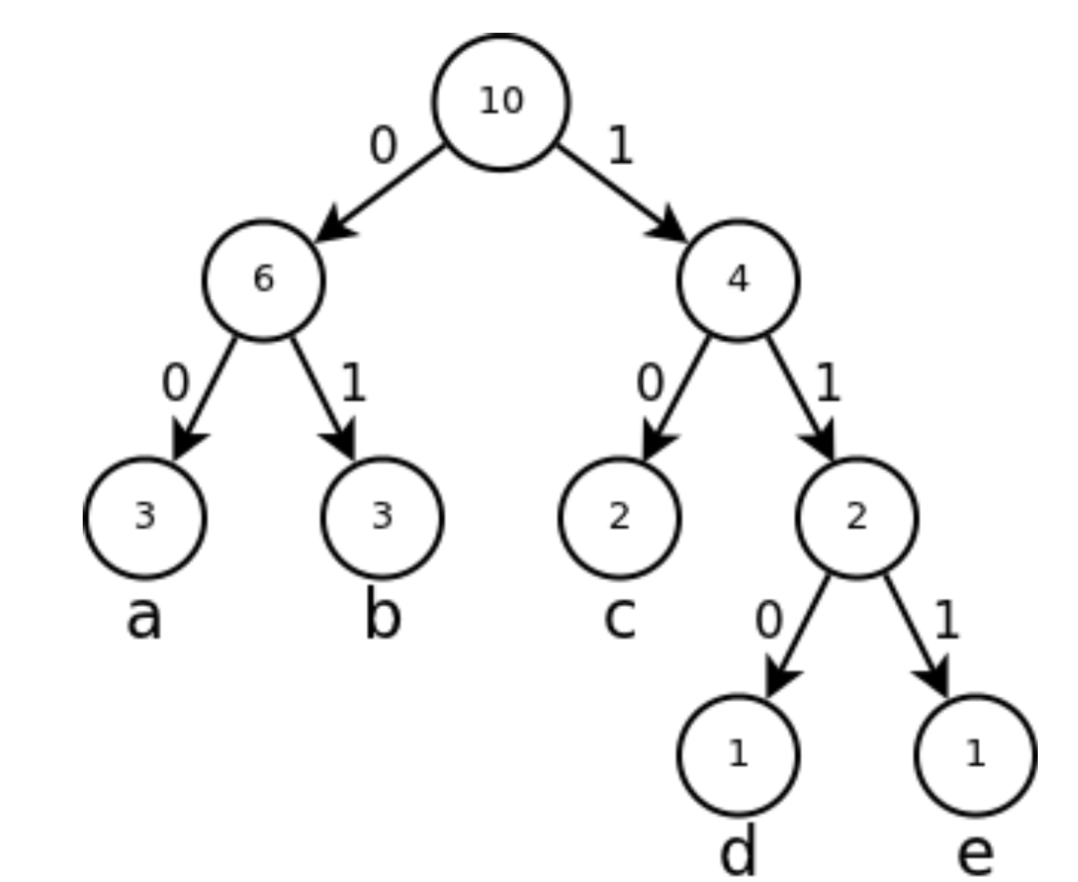
\includegraphics[width = .5\linewidth]{huffman.png}
    \caption{An example Huffman tree}
    \label{fig:huffman}
\end{figure}
To retrieve the code for each symbol, we take the path from the root to the leaf symbol. The code length for a symbol at depth $D$ is $D$ bits, thus more frequently used symbols are placed at higher depths of the tree and use shorter codes. This way the length of the path to a symbol $X$ is roughly $h(x)$ (rounded up). A Huffman tree can be formed with a simple algorithm:
\begin{enumerate}
    \item Sort symbols by frequency
    \item Group the two least frequent symbols 
    \item Create a parent symbol with the sum of the two symbols, add it back to the list
    \item Repeat until no symbols remain
\end{enumerate}
Huffman encoding is ideal if the probabilities of each symbol is a power of 2, thus the path to a symbol is exactly $h(x)$, or the Shannon information of the symbol.\\[10pt]
\textit{NB}: A notable file format in bioinformatics, \textbf{CRAM}, uses a combination of Huffman, Elias-gamma, and Golomb codes to encode information about reads aligned to a reference genome.
\subsection{Run-length encoding}
Run length encoding compresses runs of identical symbols as a single symbol with an associated count. For example, the DNA sequence ``AACTTTTG" would become ``A2C1T4G". This encoding is used by the \textbf{Cigar alignment format}, which is used by the SAM format. Runs of matching nucleotides in an alignment are simply encoded as \#$N$ Matches, along with runs of insertions or deletions (which can be decoded with a reference).
\subsection{Lempel-Ziv}
The Lempel-Ziv scheme uses an adaptive dictionary, which initially stores characters of size one, but as the sequence is encoded, longer \textbf{motifs} or repeat string of characters, are given unique codes. In a biological context, the Lempel-Ziv method can detect DNA/RNA sequence repeats that are common in an encoded sequence. This method is used in the Unix ``compress" tool.
\subsection{Burrows-Wheeler}
The Burrows-Wheeler transform converts an input sequence of characters into a new representation which can be efficiently encoded. It works by generating all the rotations of the input string, and sorting the rotated strings. The last character in each rotated string is then combined to create the transformed string.
\begin{figure}[ht]
    \centering
    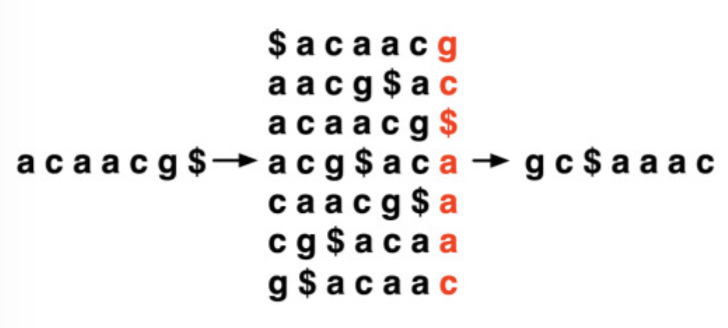
\includegraphics[width=.5\linewidth]{bw.png}
    \caption{Example of the Burrows-Wheeler Transform (\$ represents the end character)}
    \label{fig:my_label}
\end{figure}
In the transformed string, repeated substrings from the input will show up as repeated characters, which can then be efficiently encoded using a run-length encoding. This transformation is also reversible, and can thus be decoded using the same process. Compression tools like the bzip2 use this method in practice. In bioinformatics, sequence aligners like \textbf{Bowtie} and \textbf{BWA} use the Burrows-Wheeler transform to index reference genomes to efficiently align short reads.
\section{Summary}
Information theory uses concepts from probability theory and statistics to describe the information in data, which can be used to design efficient compression schemes and codes. Nucleotide sequences are also strings of data with information content, so concepts from information theory can be applied in computational biology to build efficient algorithms for analyzing and storing biological data.
\end{document}



